\documentclass[11pt]{article}
\usepackage[margin=1.1in]{geometry}
\usepackage{amsmath}
\usepackage{graphicx}
\title{Harmonic Distortion Notes:\\ The Two-Parameter Sine Model}
\author{A.~Researcher\thanks{Preliminary draft; worked example.}}
\date{October 2026}
\begin{document}
\maketitle
\begin{abstract}
We study the simplest two-parameter oscillation and ask how its amplitude and
frequency controls interact when a signal is sampled at fixed intervals.
Throughout the note the amplitude is written $a$ and the angular frequency is
written $b$; the independent variable is time, written $x$.
\end{abstract}

\section{The model}
The signal of interest is the pure sine with modulated amplitude:
\begin{equation}
  y = a \sin(bx).
  \label{eq:sine}
\end{equation}
Here $a$ controls the peak value of the signal and $b$ controls how fast the
oscillation repeats. Doubling $a$ stretches the curve vertically; doubling $b$
compresses it horizontally by one half. When $a$ is negative the curve flips.

\section{Envelope of a damped variant}
For comparison, the damped variant decays exponentially:
\begin{equation}
  u(t) = e^{-t}\cos(\omega t).
  \label{eq:damped}
\end{equation}
Both formulas are studied numerically in the accompanying worksheet; the
sweep below fixes the sampling grid and varies the two parameters of
\eqref{eq:sine}.

\section{A sampled trace}
A short sample of the model with $a = 1.5$ and $b = 2$ is plotted in
Figure~\ref{fig:trace}.
\begin{figure}[h]
  \centering
  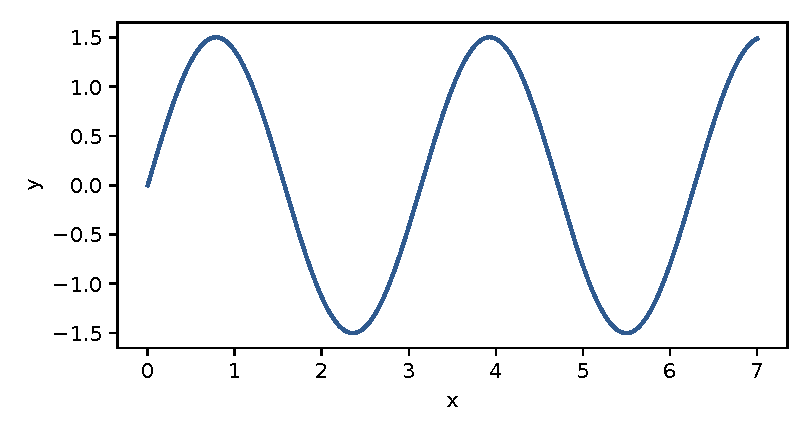
\includegraphics[width=0.62\linewidth]{plot.pdf}
  \caption{One period-sampled trace of \eqref{eq:sine} at $a=1.5$, $b=2$.}
  \label{fig:trace}
\end{figure}

\end{document}
